%\documentclass{emulateapj}
\documentclass[twocolumn,apj,numberedappendix]{emulateapj}
\usepackage{hyperref}
\newcommand{\vdag}{(v)^\dagger}
\newcommand{\myemail}{tleung@astro.cornell.edu}
\newcommand{\Msun}{\mbox{$M_{\odot}$}}
\newcommand{\Rsun}{\mbox{R$_{\odot}$}}
\newcommand{\Lsun}{\mbox{L$_{\odot}$}}
\newcommand{\rarr}{$\rightarrow$}
\newcommand{\CO}{\mbox{CO($J$ = 3 $\rightarrow$ 2) }}
\newcommand{\Lp}{\mbox{$L^{\prime}_{\rm CO(1-0)}$}}
\newcommand{\LpU}{\mbox{K km s$^{-1}$ pc$^2$}}
\newcommand{\eg}{{\sl e.g.,~}}
\newcommand{\ie}{{\sl i.e.,~}}
\newcommand{\pmOne}{$^{-1}$}
\newcommand\tna{\,\tablenotemark{a}}
\newcommand\tnb{\,\tablenotemark{b}}
\newcommand\tnc{\,\tablenotemark{c}}
\newcommand\tnd{\,\tablenotemark{d}}
\newcommand\tne{\,\tablenotemark{e}}
\newcommand\tnf{\,\tablenotemark{f}}
\newcommand\tng{\,\tablenotemark{g}}

%\slugcomment{{\sc Accepted to ApJ:} August 1, 2006}
\usepackage{amsmath}
\usepackage{natbib}
\citestyle{aa}
\shorttitle{Study of a strongly lensed type-2 quasar host SMG at $z$ = 2.221}
%\shortauthors{Leung and Riechers}

\begin{document}
\title{\CO observation in a strongly lensed type-2 quasar host SMG at $z$ = 2.221 with
continuum detection in the lensing FR-II galaxy 3C220.3}
\author{No name}
%\author{T. K. Daisy Leung\altaffilmark{1} and Dominik R. Riechers}
%\affil{Astronomy Department, Cornell Unviersity}
%\altaffiltext{1}{tleung@astro.cornell.edu}

\begin{abstract}
We report the detection of \CO line emission in SMM J0939+8315 ($z$ = 2.221), a
strongly lensed high-redshift submillimeter galaxy (SMG) hosting a type-2 quasar using
the Combined Array for Research in Millimeter-wave Astronomy (CARMA). This lensing system consists of a
foreground radio galaxy and a companion galaxy at $z$ = 0.685. A lensing magnification of $\mu_{\rm 1 mm}$ = 9.74 $\pm$ 1.4 amplified the intrinsic luminosities of the CO emission. This allows us to place constraints on the intrinsic properties
of the cold gas and dust in the interstellar medium (ISM) of the background quasar host SMG. Prior to correcting for lensing 
amplification, we measure the
velocity-integrated \CO line intensity of $I_{\rm CO(3-2)}$ = (14.6 $\pm$ 0.9) Jy km s\pmOne,
corresponding to a lensing-corrected CO($J$ = 1 \rarr 0) line luminosity of \Lp = (4.1 $\pm$ 
0.9) $\times$ 10$^{10}$ \LpU. This
translates to a molecular gas mass of $M_{\rm gas}$ = 3.3 $\times$ 10$^{10}M_\odot$, assuming a conversion
factor of $\alpha_{\rm CO}$ = 0.8 \Msun (\LpU)\pmOne. We report marginally resolved continuum 
emission from the foreground radio galaxy 3C220.3 with peak flux density of $S_\nu$ = 5.56 $\pm$ 0.54 mJy
 at 104 GHz, allowing us to put constraints on the spectral energy distribution (SED) of this galaxy. We 
fit
 both an optically thick and optically thin modified blackbody models to the SED of the SMG using existing
infrared photometric data. Our SED fitting favours an optically thick model, yielding dust mass of $M_{\rm
dust}$ = 50.5$^{20.4}_{-20.2}$ $\times$ 10$^8$\Msun, and total infrared (IR) luminosity of $L$ = 88.5$^{+2.6}
_{-2.6}\times$10$^{12}$\Lsun, prior to lensing correction. We conclude that the properties (\eg gas mass, gas mass 
fraction, SFR) of the molecular gas reservoir in SMM
J0939+8315 based on our \CO observation is similar to other high redshift
SMGs. \\
NEED TO  FIX: 
report SFR, gas-to-dust ratio.. Comparison, etc. 
\end{abstract}
\keywords{galaxies: formation --- galaxies: high-redshift --- submillimeter: galaxies}

\section{Introduction}\label{sec:intro}
Submillimeter-selected galaxies (SMGs) are predominantly found at redshift $z \sim$ 1-3, during the epoch of stellar mass and 
galaxy assembly. These galaxies are luminous in submillimeter (submm) due to the re-radiation from the dust components in the
 far-infrared (FIR) wavelengths. Followup observations of SMGs discovered in large sky surveys (e.g., HERMES, HATLAS) with sub-(mm) facilities have led to growing consensus
  of the observable properties of SMGs (cite). SMG is a population of high-redshift galaxy that are typically dusty, gas-rich, 
  and luminous ($\gtrsim$ 10$^{12}$ \Lsun) in infrared with high star formation rates ($\gtrsim $ 500 \Msun yr\pmOne). (e.g., Lagache et al. 2005, cite more recent). \par
  To characterize the physical properties of the gas reservoirs in the ISM where active star formation takes place, carbon monoxide (CO) rotational lines have been commonly used as tracers due to the high abundance of this molecule in the ISM as well as its low excitation energy, the ground state transition line thereby directly probes the cool gas that is essential to fuel star formation \citep{Carilli13a}. Recent observations of the CO line of SMGs at $z \sim$ 1-3 have  
provided evidence that SMGs have large gas reservoirs typical of \textgreater 10$^{10}$\Msun. In most cases, detailed studies are carried out on SMGs that are gravitationally lensed, lensing amplifies the intrinsic luminosities of these sources, making them the brightest unveiled in large sky surveys (Negrello 10, cite). \par
One of such lens system has a peculiar configuration consisting of a SMG, SMM J0939+8315 (hereafter SMM J0939), hosting a 
type-2 quasar at $z$ = 2.221. SMM J0939 is being strongly lensed by a double-lobed Fanaroff-Riley Class II (FR-II) \citep*{Fanaroff74} radio galaxy (3C220.3) which has a 
companion galaxy B at $z$ = 0.685, separated by 1\farcs5. SMM J0939 is currently
the brightest known lensed
SMGs, with lensing-magnified flux density of SMM J0939 $F_{\rm 250\mu m}$ = 440 $\pm$ 15 mJy. The redshift of SMM J0939 has 
been measured through the detection of CIV 1459\AA\
 and HeII 1640\AA\
line emissions \citep[hereafter H14]{Haas14}, these line detections provide conceivable evidence of AGN activity in this SMG, as well as the identification of a type-2 quasar. 

In this paper, we present the detection of \CO line emission obtained with the Combined
Array for Research in Millimeter Astronomy (CARMA) in the background SMG
SMM J0939 at $z$ = 2.221. The underlying radio continuum at 104 GHz allows us to put constraints on the SED of the 
foreground radio galaxy. This paper is organized as follows: in \S \ref{sec:obs}, we describe the
observations of the \CO line emission with CARMA; in \S \ref{sec:res}, we report the
detection of the CO line in the background galaxy as well as the continuum in the foreground galaxy; in \S
\ref{sec:Lens}, we present our lens modeling analysis; in \S \ref{sec:SED}, we perform SED fitting to 3C220.3
and SMM J0939 and derive the intrinsic properties of the interstellar medium (ISM) in the SMG; in \S \ref{sec:conclusions}, we
conclude our findings by comparing to other SMGs at similar redshifts.

We adopt a standard $\Lambda$CDM cosmological model throughout this paper, with H$_0$= 69.32 km Mpc\pmOne
s\pmOne, $\Omega_{\rm M}$ = 0.286, $\Omega_\Lambda$=0.713, based on WMAP9 results \citep{Hinshaw13a}.
The luminosity distances at $z$ = 0.685 and $z$ = 2.221 are 4214 Mpc and 19052 Mpc, respectively; 1$\arcsec$
corresponds to 8.406 kpc at $z$ = 2.221, and 7.169 kpc at $z$ = 0.685.

\section{Observations}\label{sec:obs}
\subsection{CARMA} \label{sec:carmadata}
Observations of the \CO rotational transition ($\nu_{\rm rest}$ = 345.7959899 GHz),
redshifted to $\nu_{obs}$ = 107.357 GHz (2.794 mm) towards the background galaxy SMM
J0939+8315 ($z$ = 2.221) were carried out using CARMA (programme ID: cf0142; P.I.: D. Riechers).
We used the 3mm receivers with a bandwidth of 3.75 GHz in each sideband, at 5.208 MHz ($\sim$14.5 km s\pmOne)
resolution to cover the \CO line and the underlying 2.877 mm continuum emission. The CO($J$ = 3 
\rarr 2) line was placed on the
upper sideband with the local oscillator frequency tuned to $\nu_{\rm LO}$ = 104.2609 GHz.
Observations were carried out under good
weather conditions in the E array configuration on 2014 July 12. This resulted in 1.56 hours of 15 antenna-
equivalent on-source time after discarding unusable visibility data.
The nearby source J1039+811 (0.65Jy) was observed every 20 minutes for
pointing, amplitude, and phase calibration. Mars was observed as the primary
absolute flux calibrator and the quasar 3C273 was observed as the secondary
flux calibrator. J0927+390 was observed for bandpass calibration, yielding $\sim
$15\% calibration accuracy.
The {\sc MIRIAD} package was used to calibrate and analyze the visibility data, which are deconvolved and imaged using
the CLEAN algorithm with ``natural" weighting, this yields a synthesized clean beam size of 13$\farcs$57 $\times$ 
5\farcs77 . The final rms noise is $\sigma$ = 0.7 Jy km s\pmOne $\rm beam^{-1}$ over
a channel width of 135.4 MHz (corresponding to $\sim$378.1 km s\pmOne). The continuum image is created by
averaging over all the line-free channels, this yields a synthesized clean beam size of 16\farcs67 $\times$ 7\farcs17 and a 
rms noise of 0.55 mJy beam\pmOne.

% mom0 map channels [72, 85], each channel is 29.088 km/s, i.e. total velocity range is 378.144 km/s, which is 135.408 
%MHz
\section{Results}\label{sec:res}
\subsection{New results: Continuum Emission} 
Averaging over all the line-free channels, we detect a 10$\sigma$ continuum emission at an averaged frequency of $\nu_{cont}$ = 104.2106 GHz (2.877 mm) in the observed-frame, corresponding to $\sim$2.79 mm at $z$ = 0.658. In this lens system, the 
foreground galaxy (3C220.3) is radio-loud, we thus expect the continuum to be dominated by emissions from the foreground galaxy. We use CASA's {\sc imfit} task to estimate the peak position of the continuum emission, the deconvolved source size is 8\farcs72 $\pm$ 0\farcs69 $\times$ 3\farcs87 $\pm$ 1\farcs60, and the integrated flux density is 7.18 $\pm$ 0.69 mJy. At the peak position of the continuum emission, the peak flux density is S$_\nu$ = 5.56 $\pm$ 0.54 
mJy beam\pmOne.
In Figure \ref{fig:cont}, we show the continuum emission at 104 GHz overlaid on the 9 GHz continuum measurement reported by \citet{Haas14}. This figure demonstrates that at the resolution of our observation, the continuum detection is marginally resolved, it is therefore plausible that both non-thermal and thermal emissions from the lobes and the radio core contribute to the integrated flux density in our measurement.

\begin{figure*}[tbph]
\centering
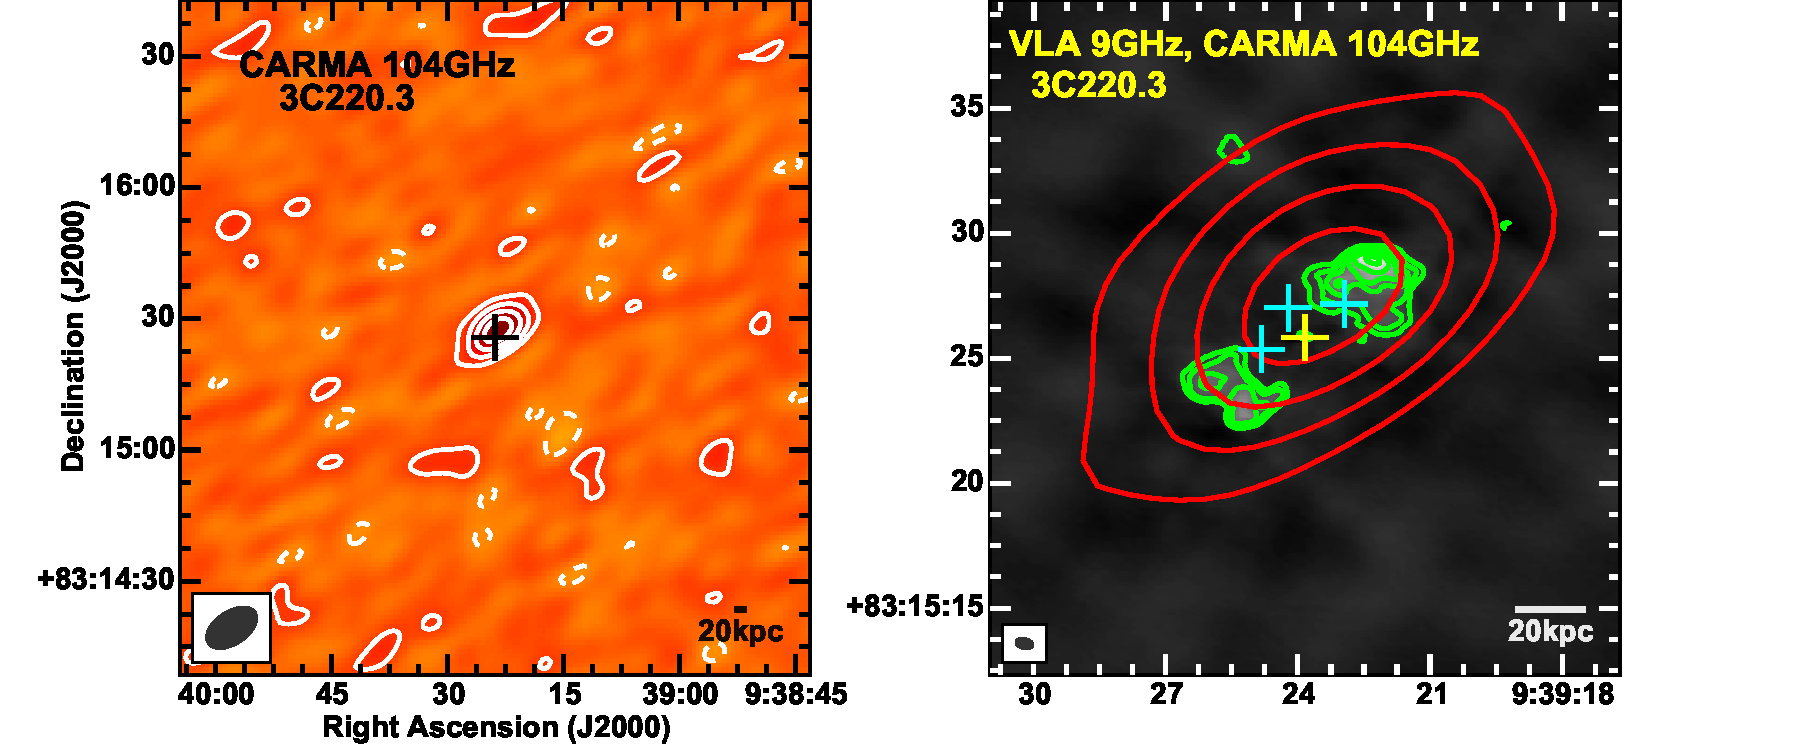
\includegraphics[width=0.80\textwidth]{Figure/ContPanel}
\caption{The central cross on each image indicates the position of the radio core of 3C220.3. Contour levels of the 9 GHz continuum 
emission start at $\pm$4$\sigma$ of $\sigma$ = 0.0641 mJy beam\pmOne and increment at steps of $\pm$2$^n\sigma$, 
where n is positive integers; contour levels of the 104 GHz continuum emission start at $\pm$3$\sigma$, incrementing at steps 
of $\pm$1$\sigma$ of 0.5 mJy beam\pmOne.
Left: Contour map of the 104 GHz continuum emission in 3C220.3. The beam size is 16\farcs67 $\times$ 7\farcs17, at P.A. = 
-58$\degr$, as indicated in the bottom left corner. Right: Contours of the CARMA 104 GHz continuum emission (red) from the 
foreground radio galaxy 3C220.3 overlaid the 9 GHz emission (green) (H14). The rms in the 9GHz image is $\sigma$ 
= 0.0641 mJy beam\pmOne. The synthesized beam size of the VLA observations is 0$\farcs$60 $\times$ 0$\farcs$23 at P.A. 
76$\degr$. 
\label{fig:cont}}
\end{figure*}

\subsection{New results: \CO line emission}
We detect \CO line emission toward the background SMG SMM J0939. Figure \ref{fig:mom0} shows the line profile at the peak position of the CO emission. Fitting a four-parameter single-component Gaussian to the spectrum yields a peak flux density of 19.9 $\pm
$ 2.2 mJy superimposed on a continuum level of 3.46 $\pm$ 0.40 mJy, and full width at half-maximum (FWHM) of 541.65 $\pm$ 31.91 km s\pmOne. 
The spatial extent of the SMG is shown in the SMA 1 mm dust continuum in Figure \ref{fig:mom0}, the 
synthesized beam size of the SMA observation is 1\farcs42$ \times $1\farcs16, at P.A. -34.0\degr. As such, the \CO detection in the SMG is spatially unresolved. We construct a velocity-integrated (0th moment) map of the \CO 
emission using the continuum-subtracted data in the visibility plane, this results in velocity-integrated \CO line flux of $S_{\rm CO}$ = 14.6 $\pm$ 0.9 Jy km s\pmOne over a velocity range of $\Delta v$ = $\sim$378.1 km s\pmOne, the uncertainty does not include $\sim$ 15\% calibration uncertainty. We ignore the primary beam correction given that the source is close to the phase center, and that the source is unresolved (\ie much smaller than the primary beam size).

\begin{figure*}[tbph] 
\centering
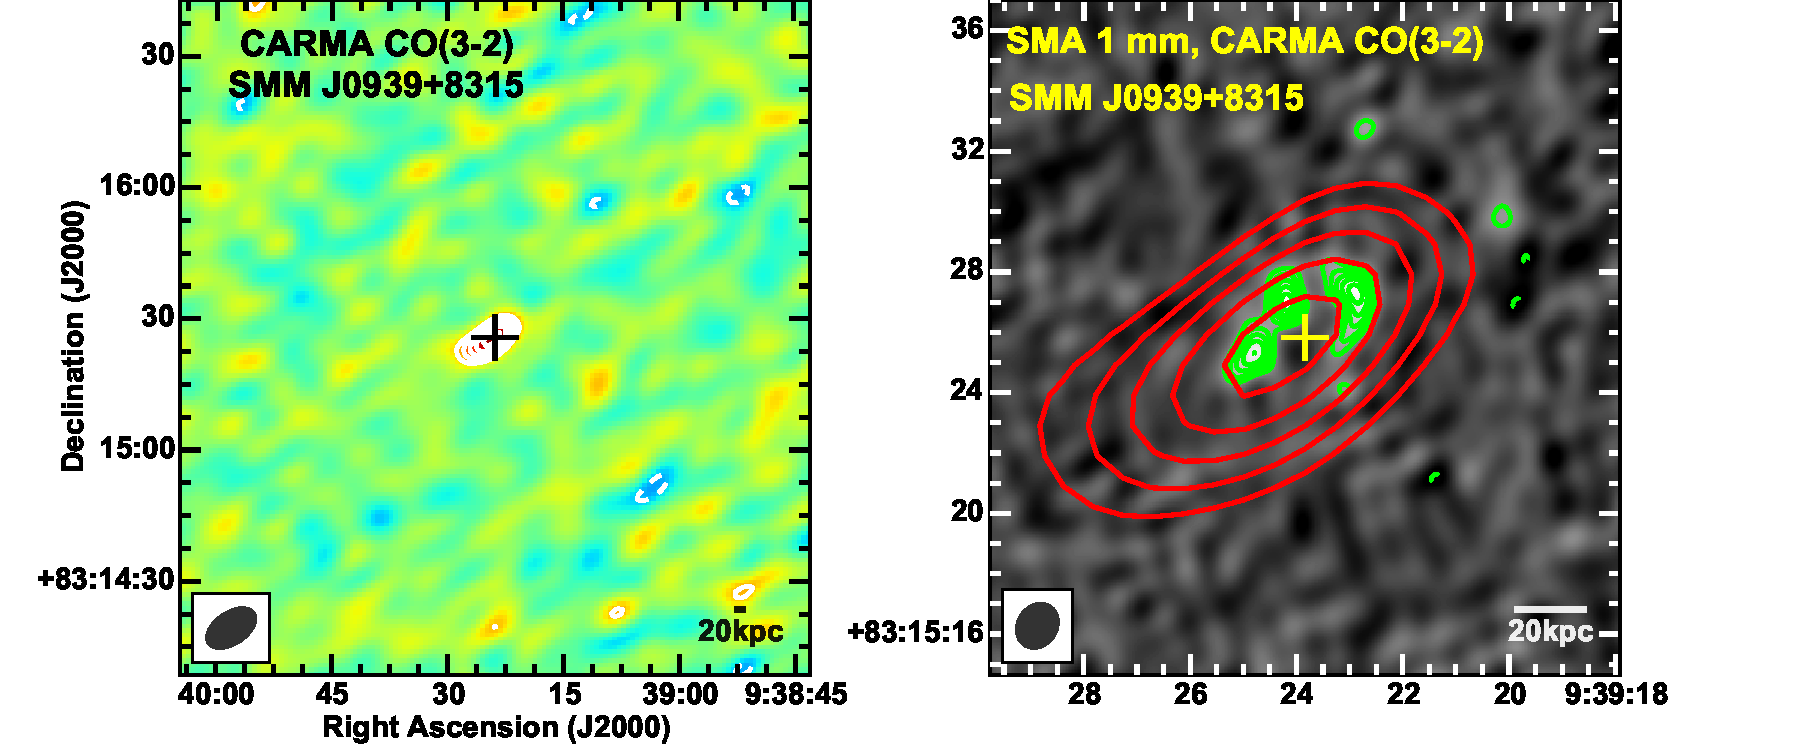
\includegraphics[width=0.8\textwidth]{Figure/LinePanel}
\includegraphics[width=0.65\textwidth]{Figure/peak28_WiderSpectrum}
\caption{The central cross on each image sets the coordinates for alignment between plots. The contour starts at $\pm$3$\sigma$, 
incrementing at
steps of $\pm$1$\sigma$. Top Left: Continuum-subtracted moment-0 map of the \CO line emission in 
the background SMG with $\sigma$ = 0.7 Jy km s\pmOne beam\pmOne. The angular resolution is 13$\farcs$57 $\times$ 
5\farcs77, as shown in the bottom left corner. 
Top Right: Contours of \CO emission (red) overlaid on the SMA 1 mm dust continuum (green) with $
\sigma$ = 0.84 mJy beam\pmOne. The beam size of the SMA data is 1\farcs42$ \times $1\farcs16, P.A. -34\degr, as shown 
in the bottom left corner. From this image, it is apparent that the extent of the background SMG is smaller than the beam 
size of the CARMA observations, hence the \CO line detection is spatially unresolved. Bottom: 
The spectrum at the CO emission peak position with spectral resolution of $\Delta v$ $\sim$29.1 km s\pmOne.
Solid black line shows the Gaussian fit to the \CO line profile. Yellow histogram shows the 
flux density as a function of velocity offset, where 0 km/s corresponds to $z$ = 2.221. \label{fig:mom0}}
\end{figure*}


\section{Analysis}
\subsection{Lens Modelling} \label{sec:Lens} 
To study the intrinsic properties of the background galaxy, we determine the magnification factor by performing
lens modeling using the SMA 1 mm archival data of this system. The lens modeling is carried out in the visibility
(uv-) plane using the updated version\footnote{commit: 7aee6276} of the publicly available software {\sc uvmcmcfit}
\citep{Bussmann15a}. The code uses affine-invariant Markov chain Monte Carlo (MCMC) to sample the posterior
probability density function (PDF) of the model parameters. In our lens model, the surface mass densities of both
lenses are represented by singular isothermal ellipsoid (SIE) profiles, and the source is assumed to have an
elliptical Gaussian profile. The code does not include an external shear parameter. \newline
We fix the phase center to coordinates ($\alpha$, $\delta$) (J2000) = (144.84809\degr, 83.25725\degr), the
offset positions of the lenses and source are referenced to this phase center. The primary lens (3C220.3) is
described by 5 free parameters: the angular offset relative to
the chosen phase center in the image ($\Delta \alpha_{\rm
lens0}$ and $\Delta \delta_{\rm lens0}$), the angular Einstein radius ($\theta_{\rm E,0}$), the
axial ratio ($q_{\rm lens0}$), and the position angle ($\phi_{\rm lens0}$). The secondary lens (companion B) is
described by 3 free parameters: $\theta_{\rm E,1}$, $q_{\rm lens1}$, and $\phi_{\rm lens1}$. The angular offset
of the secondary
lens is sampled with respect to ($\Delta \alpha_{\rm lens0}$ and $\Delta \delta_{\rm lens0}$) of
the primary lens.
The source (SMM J0939) is parameterized by
6 free parameters: the position of the source relative to the
primary lens ($\Delta \alpha_{\rm s}$ and $\Delta
\delta_{\rm s}$), the total intrinsic flux density ($S$), the
effective radius ($r_{\rm s} = \sqrt{a_{\rm s} b_{\rm s}}$), the axial
ratio ($q_{\rm s}$ =  $b_{\rm s}/a_{\rm s}$), and the position angle
($\phi_{\rm s}$).
The total number of free parameters is $N_{\rm free}$ = 14. The best-fit model is obtained by maximizing the
Gaussian likelihood function $ \mathcal{L} $ according to:
\begin{equation}
    \mathcal{L} = \sum_{u, v}\left( \frac{|V_{\rm data} - V_{\rm
    model}|^2}{\sigma^2} + {\rm log}(2 \pi \sigma^2) \right)
\end{equation}
\noindent where $\sigma$ is determined from the scatter in the visibilities within a
single spectral window (natural weighting).

We initialize the positions and the Einstein radii of both lenses, and the position of the source using the
values of the best-fit lens model \citet{Haas14} performed on Keck K-band near-infrared image. For each of
these parameters, we impose a uniform prior in the range $\in\pm$3$\sigma$, where $\sigma$ is the uncertainty
reported in their paper. The axial ratios of the lenses are restricted to $q_{\rm lens} > 0.3$. We initialize 512
walkers and 6000 steps to identify the best-fit model parameters.
\begin{figure}[!tbpH]
\centering
\includegraphics[width=0.232\textwidth]{Figure/LensedSBmap_model_goodfit0771}
\includegraphics[width=0.232\textwidth]{Figure/LensedSBmap_residual_goodfit0771}
\caption{We perform lens modeling using the latest version of {\sc uvmcmcfit} on the SMA 1 mm continuum data.
In this two lenses model, we initialize the lenses' positions using the values reported by \citet{Haas14}. Left:
Grayscale: Our best-fit model assuming an elliptical Gaussian profile for the background SMG. Magenta ellipses:
Half-light area of the background SMG. Orange Lines: Critical curves of foreground lenses. Black dots: Positions of
the two lenses. Red contours: Observed SMA 1 mm continuum. The contours start at 2$\sigma$, incrementing at
steps of $\pm$2$\sqrt{\rm 2}\sigma$. Right: Solid contours show the positive residuals at the same levels and dashed contours
show the negative residuals. \label{fig:lens}}
\end{figure}

The resulting best-fit model as shown in Figure \ref{fig:lens} shows no significant bowls in the residual
image, and the knots (lensed emission) in the observed SMA data are well-reassembled with the best-fit model.
The best-fit model yields a magnification
factor of $\mu_{\rm 1mm}$ = 9.73 $\pm$ 1.38, this is consistent the value reported by \citet{Haas14} within errors. The Einstein radii associated with the best-fit model for the two lenses are $\theta_{E}$ =
1.22 $\pm$ 0.01 (8.75 kpc at $z$ = 0.685) and $\theta_{E}$ = 0.73 $\pm$ 0.02 (5.23 kpc at $z$ = 0.685),
the corresponding masses within the Einstein radii are $M(\theta < \theta_{\rm E})$ = (4.90 $\pm$ 0.58) $\times$ 10$^{11}$ 
\Msun 
and $M(\theta < \theta_{\rm E})$ = (1.76 $\pm$ 0.33) $\times$ 10$^{11}$ \Msun, respectively. All best-fit
parameters are listed in Table \ref{tab:lensParam}.
\begin{deluxetable}{l l r}[tbpH]
\tabletypesize{\scriptsize}
\tablecolumns{3}
\tablewidth{0pc}
\tablecaption{Lens modeling results}
\tablehead{
\multicolumn{2}{c}{Parameters} &
\colhead{Best-Fit Values}
\\ \cline{1-3} \vspace{-0.05in} \\
% \tableline
\multicolumn{3}{c}{Lens 0}
}
\startdata
%\cutinhead{Lens 0}
$\Delta \alpha_{\rm lens0}$      & (\arcsec)   & 0.403 $\pm$ 0.026     \\
$\Delta \delta_{\rm lens0}$      & (\arcsec)   & -0.181 $\pm$ 0.027    \\
$q_{\rm lens0}$ \tablenotemark{a} &             & 0.446 $\pm$ 0.063     \\
$\phi_{\rm lens0}$                & (deg)       & 31.56 $\pm$ 4.15\phn  \\
$\theta_{\rm E0}$                & (\arcsec)   & 1.218 $\pm$ 0.010     \\
\cutinhead{Lens 1}
$\Delta \alpha_{\rm lens1}$       & (\arcsec)   & -0.804 $\pm$ 0.034    \\
$\Delta \delta_{\rm lens1}$       & (\arcsec)   & -1.243 $\pm$ 0.017    \\
$q_{\rm lens1}$ \tablenotemark{a} &             & 0.608 $\pm$ 0.138     \\
$\phi_{\rm lens1}$                & (deg)       & 14.2 $\pm$ 15.7\phn      \\
$\theta_{\rm E1}$                & (\arcsec)   & 0.745 $\pm$ 0.015     \\
\cutinhead{Source}
$\Delta \alpha_{\rm s}$           & (\arcsec)   &  -0.163 $\pm$  0.035   \\
$\Delta \delta_{\rm s}$           & (\arcsec)   & -0.193 $\pm$  0.048   \\
$q_{\rm s}$ \tablenotemark{a}     &             & 0.424 $\pm$ 0.237     \\
$\phi_{\rm s}$                    & (deg)       & 174.34 $\pm$ 8.89\phn \\
$r$\tablenotemark{b}              & ($\arcsec$) & 0.106 $\pm$   0.033   \\
$\mu$                             &             & 10.13 $\pm$ 1.38\phn
\enddata
% 0.377 & -0.209 & 0.446 & 33.22 & 1.223 & -0.788 & -1.26 & 0.5289 & 9.55 & 0.733 & 9.74
\label{tab:lensParam}
\tablenotetext{a}{Axial ratio}
\tablenotetext{b}{Effective Radius}
% \tablenotetext{c}{}
\tablecomments{The angular offsets listed above are with respect to $\alpha$ = 9:39:23.54, $\delta$ = 83:15:26.10 (J2000). }
\end{deluxetable}

















\subsection{SED fitting} \label{sec:SED}
\subsubsection{3C220.3}
In the theory of synchrotron emission, continuum emission from extended components of a radio galaxy decreases with increasing frequencies, and the spectrum is commonly characterized by a power law distribution $S \propto \nu^{-\alpha}$ where the spectral index $\alpha$ is $\gtrsim$ 0.5. While the contribution from extended components decreases, studies using samples of radio galaxies have suggested that the flat/inverted-spectrum of the compact radio core component rises and dominates the flux density at higher frequencies (cite). Consequently, we expect the peak flux density in our continuum detection of $S_{\rm 104GHz}$ = 5.56 $\pm$ 0.54 mJy to be dominated by the unresolved core component of the foreground FR-II. On the other hand, the integrated flux density of 7.18 $\pm$ 0.69 mJy is suggestive of a marginally resolved detection of the extended components with non-negligible emission. This is plausible given that the orientation of the synthesized beam in our observations aligns with the axis along the 
lobes of the radio galaxy, as shown in Figure \ref{fig:cont}. We investigate this disparity by fitting an SED to existing data of the total integrated flux as listed in Table \ref{tab:SEDdataRadio}, and extrapolating the fit to estimate the flux density of the lobes at the frequency of our continuum measurement. For the core, an upper limit of $<$0.17 mJy at 4.6 GHz \citep{Mullin06a}, and a clear detection of 0.8 mJy at 9 GHz (H14) is indicative of a substantially inverted spectrum of the core, although we note that these measurements are taken across epochs. All measurements are plotted in Figure \ref{fig:SED}. \begin{deluxetable}{rlrcc}[tbpH]
\tabletypesize{\scriptsize}
\tablecolumns{5}
\tablecaption{Continuum data of 3C220.3}
\tablehead{
\multicolumn{2}{c}{Frequency} &
\multicolumn{2}{c}{Flux Density} &
\colhead{Reference} \vspace{0.05in}
\\  \cline{1-5} \vspace{-0.05in} \\
\multicolumn{5}{c}{Integrated (Core \& Lobes)}
}
\startdata
    104.2 & GHz & 7.39 $\pm$ 1.42\tna        & mJy & LR15 \\
%    104.2 & GHz & 4.91 $\pm$ 0.54\tna        & mJy & This work \\
    10.7  & GHz & 270 $\pm$ 30            & mJy & KP73       \\
    10.7  & GHz & 253 $\pm$ 28            & mJy & L80       \\
    5.0   & GHz & 640 $\pm$ 100           & mJy & K69       \\
    5.0   & GHz & 636 $\pm$ 50            & mJy & L80       \\
    2.7   & GHz & 1.33 $\pm$ 0.07         & Jy  & K69       \\
    2.7   & GHz & 1.34 $\pm$ 0.10         & Jy  & L80       \\
    1.4   & GHz & 2.95 $\pm$ 0.09         & Jy  & C98       \\
    1.4   & GHz & 2.99 $\pm$ 0.06         & Jy  & P66       \\
    1.4   & GHz & 2.80 $\pm$ 0.14         & Jy  & K69       \\
    1.4   & GHz & 2.89 $\pm$ 0.09         & Jy  & L80       \\
    0.75  & GHz & 5.94 $\pm$ 0.28         & Jy  & L80       \\
    0.75  & GHz & 5.94 $\pm$ 0.21         & Jy  & P66       \\
    0.75  & GHz & 5.60 $\pm$ 0.84         & Jy  & K69       \\
    352   & MHz & 11.3 $\pm$ 0.453        & Jy  & WENSS     \\
    352   & MHz & 11.6 $\pm$ 0.464        & Jy  & WENSS     \\
    178   & MHz & 15.7 $\pm$ 2.35         & Jy  & K69       \\
    178   & MHz & 17.1 $\pm$ 1.71         & Jy  & L80       \\
    152   & MHz & 22.6 $\pm$ 0.08         & Jy  & B85       \\
    152   & MHz & 22.5 $\pm$ 0.04         & Jy  & B85       \\
    86    & MHz & 51.6 $\pm$ 9.90         & Jy  & L80       \\
    73.8  & MHz & 37.5 $\pm$ 3.82         & Jy  & C07       \\
    38    & MHz & 49.6 $\pm$ 4.96         & Jy  & L80       \\
    38    & MHz & 40.2 $\pm$ 6.30         & Jy  & K69       \\
    37.8  & MHz & 60.7 $\pm$ 6.07         & Jy  & H95       \\
    17.8  & MHz & 64.9 $\pm$ 6.49         & Jy  & H95			\\
\cutinhead{Core Only}
    104.2 & GHz & $<$ 2.29 		      & mJy & LR15 \\
    9.0   & GHz & 0.80  $\pm$ 0.06    & mJy & H14       \\
    4.86  & GHz & $<$ 0.17            & mJy & M06       \\
\enddata
\label{tab:SEDdataRadio}
\tablenotetext{a}{Integrated flux density. Peak flux density of the continuum emission is 4.93 $\pm$ 0.31 mJy beam\pmOne}
%\tablenotetext{b}{Core only}
\tablenotetext{$\dagger$}{www.astron.nl/wow/testcode.php?survey=1}
%\tablecomments{References.~}
\tablerefs{
B85 = \citet{r2728};
C98 = \citet{r16};
C07 = \citet{r30};
H95 = \citet{r33-34};
H14 = \citet{Haas14};
K69 = \citet{r11-14-18-22-25-32};
KP73 = \citet{r9};
L80 = \citet{r10-13-15-19-20-26-29-31};
LR15 = this work;
M06 = \citet{Mullin06a};
P66 = \citet{r17-21};
WENSS = \citet{r23-24}$^\dagger$
}
\end{deluxetable}
















Following Equation (1) in \citet{Cleary07a}, the fit to the lobes can be expressed as a parabolic function:
\begin{equation}
\log F_{\nu}^{\mathrm lobe} (\nu) \propto - \beta\ (\log\ \nu - \log \nu_{t})^2  + \log (\exp({\frac{\nu}{\nu_c^{\mathrm lobe}}}))
\end{equation}
where $\beta$ is a parameter representing the bending of the parabola, $\nu_t$ is the frequency at which the optical depth of the synchrotron emitting plasma reaches unity, and $\nu_v^{\rm lobe}$ is the frequency corresponding to the cutoff energy of the lobe plasma energy distribution. 

The resulting fit is shown in Figure \ref{fig:SED}, the extrapolated flux density at 104 GHz is consistent with the peak flux density of our continuum measurement. The 10$\sigma$ detection of the continuum thereby suggests
non-negligible contributions from the lobes, and the peak flux density therefore does not appear to be dominated by the core 
emission. Furthermore, the contours of the 104 GHz continuum are
centered on the northern lobe as illustrated by the overlay image in Figure \ref{fig:cont}, this further supports our argument. This finding is consistent with a recent study by \citet{Hardcastle08a}, where a few radio galaxies blah blah. At the resolution of our observation, it is unclear whether the integrated flux is dominated by the hotspot or the lobes. 

\begin{figure}[!tbph]
\centering
\includegraphics[width=0.5\textwidth]{Figure/3C220_3FullSED}
\caption{The SED of 3C220.3 and SMM J0939 including the new measurements presented in this paper. 
Black dots represent existing data of 3C220.3 (see table \ref{tab:SEDdataRadio}). Red dots at 104 GHz corresponds to 
our continuum measurements (integrated, peak, and difference). The purple line corresponds to the parabolic function we 
fit to the data associated with the radio galaxy following \citet{Cleary07a}. The dashed purple line and 
the solid cyan line correspond to the best-fit SED models of the background SMG. The photometric data of the SMG are reported by \citet{Haas14}. \label{fig:SED}}
\end{figure}

\subsubsection{SMM J0939+8315} 
To constrain the dust and gas properties in the ISM of SMM J0939, we perform SED fitting on the
photometric data obtained with {\it Herschel}/PACS and SPIRE, at wavelengths
between observed-frame 70 \micron-1000 \micron, and interferometric data with SMA at 1 mm (H14). We use the publicly
available software {\sc mbb\_emcee} to perform SED fitting, the code uses an affine-invariant Markov chain Monte
Carlo (MCMC) approach, the details are described by \citet{Riechers13a} and \citet{Dowell14a}. The
functional form of the fit comprises of a modified blackbody function with a power law S$_{\lambda} \propto \lambda^\alpha
$ attached to the blue
side.
We fit both an optically thick and optically thin model. In the optically thick case, the wavelength $
\lambda_0$ = $\frac{c}{\nu_0}$ is an additional parameter which represents where the optical
depth $\tau_{\nu}$ = ($\nu$/$\nu_0$)$^\beta$ reaches unity. Thus, the functional form of the modified blackbody
in the optically thick regime is as follows:
\begin{equation}
\rm S_{\lambda} \propto \frac{(1-exp^{-(\frac{\lambda_0 (1+z)}{\lambda})^{\beta}})(\frac{c}{\lambda})^3}
{exp^{\frac{hc}{\lambda\rm{kT/(1+z)} } }-1}
\end{equation}
and in the optically thin regime, the functional form reduces to:
\begin{equation}
\rm S_{\lambda} \propto \frac{(\frac{c}{\lambda})^{\beta+3}}{exp^{\frac{hc}{\lambda\rm{kT/(1+z)}}}-1}
\end{equation}
where $T$ is the rest-frame characteristic cold dust temperature, $\lambda_0$ is rest-frame wavelength
where the optical depth reaches unity, $\beta$ is the dust emissivity (or spectral index of the dust extinction
curve), and $\alpha$ is the power law spectral index. The overall fit is normalized using the observed-frame 500
$\micron$ flux density, hence this becomes an additional parameter in the fit. In both models, we impose an upper limit on $
\lambda_0$ to 2000 \micron, and the observed-frame dust temperature $T/(1+z)$ to 60 K. We fix the upper limit on 
$\beta$ to be 3.0 and 2.2 for the optically thin model and optically thick model, respectively.

\begin{deluxetable}{ccc}[tbpH]
\tabletypesize{\scriptsize}
\tablecolumns{3}
\tablecaption{SED fitting results}
\tablehead{
\colhead{Parameters}                  &
\colhead{Optically Thick}       &
\colhead{Optically Thin}
}
\startdata
$\chi^2$ & 2.25 & 5.31 \\
D.O.F & 2 & 3 \\
$T_{\rm d}$ (K) & 60.91$^{+1.08}_{-1.31}$ & 51.95$^{+1.26}_{-1.21}$ \\
$\beta$ & 1.35$^{+0.57}_{-0.53}$ & 0.7$^{+0.24}_{-0.26}$ \\
$\alpha$ & 3.05$^{+0.31}_{-0.40}$ & 2.76$^{+0.23}_{-0.23}$ \\
%$\lambda_0$(1+$z$) ($\micron$) \tablenotemark{c} & 722.81$^{+276.88}_{-398.67}$ & --- \\
$\lambda_0$ ($\micron$) \tablenotemark{e} & 224.41$^{+85.96}_{-123.77}$ & --- \\
$\lambda_{\rm peak}$ \tablenotemark{c}\micron & 254.7$^{+6.2}_{-6.1}$ & 301.4$^{+29.0}_{-30.1}$ \\
$f_{\rm norm, 500 \micron}$ mJy  \tablenotemark{c} & 255.79$^{+16.67}_{-16.31}$ & 244.25$^{15.28}_{15.30}$ \\
$L_{\rm (8-1000)\micron}$ [10$^{12}$ L$_\sun$] \tablenotemark{d} & 88.52$^{+2.62}_{-2.63}$ & 89.15 \\
$M_{\rm d}$ [10$^8$ M$_\odot$] \tablenotemark{b} & 50.47$^{+20.42}_{-20.15}$ & 25.74$^{+3.88}_{-5.49}$
\enddata

% Optically thick & 18.91 & 1.35 & 722.81 & 3.05 & 254.7 & 88.52 & 50.47 \\
% Optically thin &  16.13 & 0.7 & N/A   & 2.76 & 301.4 & 89.15 & 25.74

\label{tab:mbb}
\tablenotetext{a}{The observed-frame wavelength where the dust becomes optically thick}
\tablenotetext{b}{Assuming standard absorption mass coefficient $\kappa$=2.64 m$^2$ kg$^{-1}$ at $\lambda$=125.0 $\micron$ (Dunne et al. 2003), without lensing correction}
\tablenotetext{c}{observed-frame}
\tablenotetext{d}{rest-frame 8-1000 $\micron$ without lensing correction}
\tablenotetext{e}{The rest-frame wavelength where the dust becomes optically thick, upper limit is 2000 $\micron$}
\tablecomments{Errors are $\pm$1$\sigma$}
\end{deluxetable}

% thick_500_500.log
% T/(1+z): 18.91 +1.09 -1.31 (low lim: 1.00 upper lim: 60.00) [K]
% beta: 1.35 +0.57 -0.53 (low lim: 0.10 upper lim: 2.20)
% fnorm: 255.79 +16.67 -16.31 (low lim: 0.03) [mJy]
% lambda0 (1+z): 722.81 +276.88 -398.67 (low lim: 1.00 upper lim: 3049.15) [um]
% alpha: 3.05 +0.31 -0.40 (low lim: 0.10 upper lim: 20.00)
% Lambda peak: 254.7 +6.2 -6.1 [um]
% L_IR(8.0 to 1000.0um): 88.52 +2.62 -2.63 [10^12 L_sun]
% M_d(kappa=2.64, lam=125.0um): 50.47 +20.42 -20.15 [10^8 M_sun]
% Number of data points: 7
% ChiSquare of best fit point: 2.25

% note using beta upper limit 3.0, getting very different beta, and dust mass
% Fit results:
% T/(1+z): 19.75 +0.56 -0.53 (low lim: 1.00 upper lim: 60.00) [K]
% beta: 1.91 +0.76 -0.76 (low lim: 0.10 upper lim: 3.00)
% fnorm: 267.13 +16.03 -15.98 (low lim: 0.03) [mJy]
% lambda0 (1+z): 1012.99 +142.79 -275.29 (low lim: 1.00 upper lim: 3049.15) [um]
% alpha: 3.64 +0.08 -0.86 (low lim: 0.10 upper lim: 20.00)
% Lambda peak: 255.6 +6.3 -6.2 [um]
% L_IR(8.0 to 1000.0um): 88.02 +2.85 -2.85 [10^12 L_sun]
% M_d(kappa=2.64, lam=125.0um): 108.23 +32.00 -63.67 [10^8 M_sun]
% Number of data points: 7
% ChiSquare of best fit point: 2.25
% Saving results to thick_testbeta.h5

% thin_testSMA
% T/(1+z): 16.13 +1.26 -1.21 (low lim: 1.00 upper lim: 60.00) [K]
% beta: 0.70 +0.24 -0.26 (low lim: 0.10 upper lim: 3.00)
% fnorm: 244.25 +15.28 -15.30 (low lim: 0.03) [mJy]
% alpha: 2.76 +0.23 -0.23 (low lim: 0.10 upper lim: 20.00)
% Lambda peak: 301.4 +29.0 -30.1 [um]
% L_IR(8.0 to 1000.0um): 89.15 +2.48 -2.51 [10^12 L_sun]
% M_d(kappa=2.64, lam=125.0um): 25.74 +3.88 -5.49 [10^8 M_sun]
% Number of data points: 7
% ChiSquare of best fit point: 5.31

The best-fit values in both regimes are listed in Table \ref{tab:mbb}, and the correlation plots are available in appendix. The best-fit solution of an optically thin
model corresponds to $\chi^2$ = 5.31 with 3 degrees of freedom, whereas that of an optically thick model
corresponds to $\chi^2$ = 2.25 with 2 degrees of freedom, suggesting a better fit than the optically thin
model. In the subsequent analysis, we employ the inferred values from the optically thick model.
The best-fit solution yields a far-infrared (FIR) luminosity of $L_{\rm FIR (42.5-122.5\micron)}$ = 53.33$^{+1.14}_{-1.13}\times$10$^{12}$\Lsun, and a total infrared (IR) luminosity of $L_{\rm IR (8-1000 \micron)}$ = 88.52$^{+2.62}_{-2.63}\times$10$
^{12}$\Lsun. Assuming a dust absorption coefficient of $\kappa_{\nu}$ = 2.64 m$^2$ kg\pmOne at 125.0 $
\micron$ \citep{Dunne03a}, we derive the dust mass using the following expression:
\begin{equation}
M_{\rm dust} = S_{\nu} D_{L}^2 [(1 + z) \kappa_{\nu} B_{\nu}]^{-1} \tau_{\nu} [1-
\exp(-\tau_{\nu})]^{-1}
\end{equation}
where $S_{\nu}$ is the flux density, $D_{\rm L}$ is the luminosity distance, $\kappa_{\nu}$ is the dust
absorption coefficient, $\tau_{\nu}$ is the optical depth, and $B_{\nu}$ is the Planck function,
all quantities are expressed in the observed-frame. We find a dust mass of $M_{\rm dust}$ =
50.47$^{20.42}_{-20.15}\times$10$^8$\Msun, the uncertainties do not include those of $\kappa_{\nu}$. These values are based on SED fitting to the photometric data, i.e. prior
to lensing correction.
With the limited amount of data in the FIR, $M_{\rm dust}$ is weakly constrained; in another optically thick model where the upper limit of $\beta$ is set to 3.0, all fitting parameters of the best-fit solution is similar to those using an upper limit of 2.2, vary at most blah\% except for $\lambda_0$, which blah blah, the dust mass is boosted by a factor of $\sim$2. 

\subsection{Molecular gas mass}
The ground state CO transition line, CO($J$ = 1 \rarr 0) has been used as a tracer of the cold molecular gas in galaxies for over a decade. For high-redshift galaxies, the CO(J$>$1) transition lines are  
, assumptions on the CO excitation conditions is required to derive the molecular gas mass using the H2 to CO relation. 

It has long been assumed that the molecular gas in the ISM of SMGs traced by CO is thermalized given their high star formation rates (e.g. Greve et al. 2005; Coppin et al. 2008; Tacconi et al. 2008). With the few SMGs with CO(1-0) and higher J co observations to date,
Recent CO(1-0) observations of SMGs have demonstrated that SMGs can indeed be subthermally excited. (Bothwell et al. 2013, Harris et al. (2010). In these galaxies with subthermal excitation at the (3-2) transition, the brightness temperature ratio between CO(3-2) and CO(1-0) is $<$ 0.8. with an average radio of R31 = 0.6 pm 0.1 \citep[\eg][]{Harris10a,Carilli10a,Swinbank2010a,Ivison11a,Ivison10d}. While these brightness temperature ratios are $\sim$0.6 in SMGs, observations of high-z quasars suggest that the host galaxies have ratios close to unity (e.g., Riechers 
et al. 2006; 2011a; Ivison et al. 2012). Since only \CO line has been detected on this object, we adopt 1 here since the source is hosting a quasar.

We derive the molecular gas mass in
this SMG assuming thermalized excitation of CO, i.e. the brightness temperature ratio 
between \CO
and ($J$ = 1 \rarr 0) is $R_{31}$ = 1 \citep[\eg][and references therein]{Riechers11a,Scott11a}
%(\eg Ivison et al. 2008, 2012). 
We calculate the CO($J$ = 1 \rarr 0) line luminosity using standard relations 
\citep[\eg][]{Solomon05a,Carilli13a}:
\begin{equation}
L^{\prime}_{\rm CO} = \frac{3.25\times10^7}{\nu_{\rm CO (3-2), rest}^2}\times \frac{D_L^2}{\mu} \times
\frac{I_{\rm CO(3-2)}} {R_{\rm 31} (1 + z)}
\end{equation}
this corresponds to $L^{\prime}_{\rm CO (1-0)}$ = (4.13 $\pm$ 0.87) $\times$ 10$^{10}$ \pmOne (\rm K km s
\pmOne pc$^2$)
after lensing correction. The inferred total molecular gas mass is therefore M$_{\rm gas}$ = (3.3$\pm$0.7) $\times
$10$^{10}$ ($\alpha$/0.8) \Msun. We assumed a conversion factor of $\alpha_{\rm CO}$ =
0.8 \Msun (\LpU)\pmOne based on empirical relations from local ULIRGs, which is typically
adopted for SMGs \citep{Bothwell13a,Tacconi10a,Daddi2010a}. 
Combining with the dust mass derived from SED fitting, the gas-to-dust
ratio is $f_{\rm gas-dust}$ = $M_{\rm gas}/M_{\rm dust}$ = 63.74 $\pm$ blah , which is in good agreement with the range 
of values found in other SMGs \citep{Coppin08a}.

% ~ 120 for MW (Coppin 2007)
% ~ 60 for typical SMG (coppin 2008)
% ~ 100 for LBG (coppin 2007)

\subsection{Star formation rate}
We derive the star formation rate (SFR) using the \citet{Kennicutt98a} relation, assuming a \citet{Chabrier03a}
stellar initial mass (IMF) function: SFR = 1.0 $\times$ 10$^{-10}\times$ ($L_{\rm IR\ or\ FIR}$). This yields SFR$_{\rm IR}$ 
= (909.12 $\pm$ 155.67) $\times\ (\mu/9.74)^{-1}$ [$M\sun$ yr\pmOne] and SFR$_{\rm FIR}$ (547.71 $\pm$ 89.28) $\times(\mu/9.74)^{-1}$ [M$
\sun$ yr\pmOne] using lensing-corrected (far-)infrared luminosities (L$_{\rm IR}$ and L$_{\rm FIR}$) derived from our SED 
fitting, and assuming negligible contributions from AGN heating.

Assuming constant SFR, the minimum time for which the starburst in SMM J0939 can be maintained at its
current SFR is approximated by the gas depletion timescale $\tau$ = $M_{\rm gas}$/SFR, which is $\tau_{\rm IR}$ = 36.33$\pm$ blah 
Myr, and $\tau_{\rm FIR}$ = 60.30$\pm$blah Myr.

Move to discussion: Compare THIS NUMBER: with other SMGs (\eg \citep{Greve05a}). 

\subsection{SFE}
The SFR per unit mass of molecular gas is commonly taken as a
measure of the star formation efficiency, SFE = SFR/$M_{\rm gas}$. We compute the ratio using lensing-corrected (far-)infrared 
luminosities ($L_{\rm IR}$ or $L_{\rm FIR}$) and CO($J$ = 1 \rarr 0) luminosity SFE = $L_{\rm F/IR}$/\Lp, this ratio makes no assumptions on the gas mass conversion factor $\alpha$ and is independent of the 
choice of IMF, however, this assumes that differential lensing effect between the CO and infrared emission is negligible.

We find a ratio of SFE$_{\rm IR}$ = 220.22 Myr\pmOne and SFE$_{\rm FIR}$ = 132.68 Myr\pmOne, which are comparable
to what is found in "typical" SMGs (tacconi et al. 2006, Riechers et al. 2010, cite).
Greve 05.

\subsection{Dynamical mass} %% check half light radius error, and comparison
We derive the dynamical mass of SMM J0939 using an isotropic virial estimator \citep[\eg][]{Engel10a}:
\begin{equation}
M_{\rm dyn} = 2.8\times 10^5\Delta \rm v_{\rm line}^ 2 R_{\rm eff}
\end{equation}
where the line width $\Delta \rm v_{\rm line}^ 2$ is based on our \CO line
measurement and $R_{\rm eff}$ is approximated with the half-light radius of the best-fit lens model. This yields $M_{\rm dyn}$ = blah, and gas-to-
dynamical mass fraction of $f_{\rm gas-to-dyn}$ = 2.03.

Compare to other. blah blah blah dynamical mass, is it consistent with molecular gas mass?

\subsection{SFR surface density}
% using dynamical mass and Eddington luminosity limit
To compute surface densities we divided half of the star formation rate or gas mass (so that no assumption of IMF) by the area subtended by the half-light (or effective) radius.


\section{Discussion And Conclusions} \label{sec:conclusions}
We present blah

A lensed SMG that is likely to be hosting a type-2 quasar, this source offers an exceptional opportunity to
investigate the gas mass and dynamics of this
poorly-studied population of high z galaxies.

In this paper, we present blah of a strongly lensed blah at z = 2.221, at the epoch of cosmic star formation (cite)
This paper focuses on a blah source J0939+8315, a lensing galaxy.
We report a detection of \CO line.
The continuum detection is marginally resolved, we place constraints on the SED of the foreground galaxy (accounting for radio 
core and lobes emission). Our CO measurement confirms the redshift of this source, which was previously measured using CIV and HeII lines (H14).

The detection of CO in SMM J0939, implying a large molecular gas reservoir, once again demonstrates the active SF in SMGs. 
The large CO luminosity suggests that a signification fraction of the FIR luminosity comes from SF, providing power for dust to re-radiate in FIR. BUt we also know that this source has an dust-enshrouded AGN, boosting the IR.
The SFR inferred from the CO measurement is common for SMGs. the large amount of molecular gas further supports the picture that SMGs are galaxies with making up most of the stellar mass in the early universe, and is responsible for galaxy evolution and formation. 

The magnification factor is blah, providing an opportunity to carry out detailed studies of the ISM in this population.

We perform SED fitting of the SMG to get M$_{\rm dust}$, L$_{\rm FIR}$ of blah, L$_{\rm IR}$ of blah, yielding SFR of 
blah . Comparing our findings to other SMGs / similar populations, we find blah, which is blah.

We compare the properties of SMM J0939 with two other SMGs with detailed studies -- HLSW-01 and the cosmic Eyelash. All sources are lensed, making spectral lines measurements relatively feasible than their fainter, un-lensed ``siblings". 

Properties and comparison with similar galaxies in Table \ref{tab:comapreSMG}
\newcommand\tnh{\,\tablenotemark{h}}
\newcommand\tni{\,\tablenotemark{i}}
\newcommand\tnj{\,\tablenotemark{j}}
\newcommand\tnk{\,\tablenotemark{k}}
\begin{deluxetable*}{l l c c c c c}[tbpH]
\tabletypesize{\scriptsize}
\tablecolumns{7}
\tablecaption{Comparison of SMM J0939 with SMGs at $z\sim$2}
\tablehead{
\multicolumn{2}{c}{SMGs}       &
\colhead{SMM J0939}  &
\multicolumn{2}{c}{HLSW-01}    &  
\multicolumn{2}{c}{Cosmic Eyelash} 
                     \\
\colhead{Quantity} &
\colhead{Unit} &
\colhead{}                     &
\colhead{}                     &
\colhead{Ref.}                     &
\colhead{}                     &
\colhead{Ref.}
}
\startdata
$z$             &                   & 2.221            & 2.957            & R11              & 2.326          &  S10 \\
$\mu_{\rm L}$         &                   & 10.1 $\pm$ 1.4    & 10.9 $\pm$ 0.7 & G11              & 37.5$\pm$4.5    &  S11 \\
$S_{\rm 250}$ & mJy & 440 $\pm$15 (H14) & 420 $\pm$ 10  & R11              & 366 $\pm$ 55  & I10             \\
$I$\tnb       & Jy km s$^{-1}$   & 10.7 $\pm$ 2.1   & 9.7 $\pm$ 0.5  & R11              & 13.2 $\pm$ 0.1 &  D11 \\
$\Delta v_{\rm FWHM}$\tnb & km s$^{-1}$ & 542 $\pm$ 32 & 350 $\pm$ 25 & R11 & $\lesssim$ 800\tnd & D11 \\
\Lp & 10$^{10}$ \LpU & 2.91 $\pm$ 0.78\tnh & 4.17 $\pm$ 0.41 & R11 & 1.7 $\pm$ 0.2 & D11 \\
$M_{\rm gas}$ & 10$^{10}$ \Msun & 2.33 $\pm$ 0.62\tnh & 3.3 $\pm$ 0.3 & R11 & 1.6 $\pm$ 0.1 & I10 \\
$L_{\rm IR}$ &  10$^{12}$ \Lsun & 9.1 $\pm$ 1.2\tnh & 14.3 $\pm$ 0.9 & C11 & 2.3 $\pm$ 0.2 & I10 \\
$M_{\rm dust}$ & 10$^8$ \Msun & 5.2 $\pm$ 2.1\tnh  & 1 - 5.2
& R11 & $\sim$4.0 & I10 \\
SFR$_{\rm IR}$\tna & \Msun yr$^{-1}$ & 874 $\pm$ 122\tnh & 1430 $\pm$ 160\tnc & C11 & $\sim$235\tnc & I10 \\
$\tau_{\rm depl}$\tng & Myr & 25.6 $\pm$ 0.6 & 23 $\pm$ 3\tnc  & R11 & 68\tne & --- \\
$f_{\rm gas-dust}$\tng &  & 47 $\pm$ 21 & 60-330 & R11 & $\sim$ 40 & I10 \\
SFE\tng  & Myr$^{-1}$ & 300 $\pm$ 10 & 340 $\pm$ 40 & R11 & 165 $\pm$ 7 & D11 \\
$M_{\rm dyn}$\tng & 10$^{10}$ \Msun & 7.4 $\pm$ 2.4 & 3.7 $\pm$ 1.8\tne\tnf & --- & 6.0$\pm$0.5 & S11 \\
$f_{\rm gas-dyn}$ && 0.32$\pm$0.14 & 0.90\tne\tnf & --- & 0.6$\pm$0.1 & S11 \\
\enddata
\label{tab:comapreSMG}
\tablenotetext{a}{Chabrier IMF}
\tablenotetext{b}{\CO}
\tablenotetext{c}{Converted theirs values derived using Salpeter IMF to Chabrier IMF}
\tablenotetext{d}{Estimated from Figure 1 in D11}
\tablenotetext{e}{We derive this using the reported values}
\tablenotetext{f}{Using CO($J$ = 5 \rarr\ 4)}
\tablenotetext{g}{Independent of lensing magnification factor $\mu_{\rm L}$}
\tablenotetext{h}{Errors include uncertainties on $\mu_{\rm L}$}
%\tablenotetext{i}{Based on 1 mm continuum}
%\tablenotetext{j}{Based on }
%\tablenotetext{k}{Based on 870 micron, CO 1-0, 6-5, and HST}
%\tablenotetext{f}{Using $L_{\rm IR} / M_{\rm gas}$}
\tablecomments{Values listed from rows 6 onwards are lensing-corrected. References.~
C11 = \citet{Conley11a};
D11 = \citet{Danielson11a};
G11 = \citet{Gavazzi11a};
I10 = \citet{Ivison10c};
R11 = \citet{Riechers11b};
S11 = \citet{Swinbank11a};
S10 = \citet{Swinbank2010a}
}
\end{deluxetable*}
















Discussion of SMG, broad, population.
look at "Lensed QSOs at high z observational, CO measurements (DB)" note

\acknowledgments

We acknowledge the WENSS team for providing the radio measurements for 3C220.3.
Facilities: \facility{CARMA}

\bibliographystyle{apj}
\bibliography{J0939}

\appendix

\begin{figure}[!tbp]
\centering
\includegraphics[width=0.90\textwidth]{Figure/posteriorPDFs}
\caption{Figure shows the marginalized posterior probabilities of each parameter in our lens modeling.
\label{fig:LensPDF}}
\end{figure}

\begin{figure}[!tbp]
\centering
\includegraphics[width=0.55\textwidth]{Figure/CorrelationPlot__thick_500_500}
\includegraphics[width=0.55\textwidth]{Figure/CorrelationPlot__thin_testSMA}
\caption{Resulting correlation plot from our SED fitting. Plots on the diagonal axes are marginalized posterior probability 
distribution of each
parameter. Off-diagonal plots are 2D histograms between parameters. Cross denotes where the best-fit value corresponds to in 
the 2D correlation plot. Top: Optically thick
model. Bottom: Optically thin model. The parameter T/(1+z) is the observed-frame characteristic dust temperature.
\label{fig:sedlikelihood}}
\end{figure}



\end{document}

